\documentclass{beamer}

%% Use package -----------------------------------------------------------------

\usepackage[T1]{fontenc}
\usepackage[utf8]{inputenc}
\usepackage{lmodern}
\usepackage{graphicx}
\usepackage[absolute,overlay]{textpos}
\usepackage{multicol}
\usepackage{listings}

%% Beamer customization---------------------------------------------------------

\usepackage{xcolor}
\usetheme{Warsaw}

%% Themes
% Outer themes
\useoutertheme{shadow}
% Rounded boxes and shadows
\useinnertheme[shadow=true]{rounded}
% Solid \item symbols
\useinnertheme{circles}

%% Custom colors
\definecolor{rltgreen}{rgb}{0,0.5,0}
\definecolor{pasteur}{RGB}{0,90,154}
\setbeamerfont{block title}{size={}}
\setbeamercolor{structure}{fg=pasteur}
\setbeamercolor{item}{fg=pasteur}

%Color of title
\setbeamertemplate{frametitle}
{
    \nointerlineskip
    \begin{beamercolorbox}[sep=0.3cm,ht=1.8em,wd=\paperwidth]{frametitle}
        \vbox{}\vskip-2ex%
        \strut\insertframetitle\strut
        \vskip-0.8ex%
    \end{beamercolorbox}
}
% Hide navigation symbols
\setbeamertemplate{navigation symbols}{}

%% Title block
\setbeamercolor*{title}{use=structure,fg=white,bg=pasteur}

%% Bottom infolines
\setbeamertemplate{footline}
{
  \leavevmode%
  \hbox{%
  \begin{beamercolorbox}[wd=.3\paperwidth,ht=2.25ex,dp=1ex,center]{author in head/foot}%
    \usebeamerfont{author in head/foot}\insertshortauthor
  \end{beamercolorbox}%
  \begin{beamercolorbox}[wd=.7\paperwidth,ht=2.25ex,dp=1ex,center]{title in head/foot}%
    \usebeamerfont{title in head/foot}\insertshorttitle\hspace*{3em}
    \insertframenumber{} / \inserttotalframenumber\hspace*{1ex}
  \end{beamercolorbox}}%
  \vskip0pt%
}
\makeatletter

%% Top infolines
\setbeamertemplate{headline}{%
\leavevmode%
  \hbox{%
    \begin{beamercolorbox}[wd=\paperwidth,ht=2.5ex,dp=1.125ex]{palette quaternary}%
    \insertsectionnavigationhorizontal{\paperwidth}{}{\hskip0pt plus1filll}
    \end{beamercolorbox}%
  }
}

%% Define Snakemake ------------------------------------------------------------

\definecolor{eclipseBlue}{RGB}{42,0.0,255}
\definecolor{eclipseGreen}{RGB}{63,127,95}
\definecolor{eclipsePurple}{RGB}{127,0,85}

\lstset{language=Python}
\lstset{
    basicstyle=\tiny\ttfamily,
    morekeywords={rule, output, shell, params, run, configfile, temp, threads, log},
    showstringspaces=false,
    commentstyle=\color{eclipseGreen}, % style of comments
    keywordstyle=\color{eclipsePurple}, % style of keywords
    stringstyle=\color{eclipseBlue}, % style of strings
}


%% Set up title ----------------------------------------------------------------

\title{Snakemake Presentation}
\author[D.Desvillechabrol \& T.Cokelaer]{Dimitri Desvillechabrol and Thomas Cokelaer}
\institute{Institut Pasteur}
\date{March 22 2016}

\begin{document}

%% Title slide -----------------------------------------------------------------

\begin{frame}[plain]
    \titlepage
    \begin{textblock*}{5cm}(4.5cm,0.3cm)
        
\includegraphics[scale=0.09]{Institut_Pasteur.png}
    \end{textblock*}
\end{frame}

%% Slides ----------------------------------------------------------------------

\section{Introduction}

\begin{frame}
    \frametitle{Workflow management}
    \begin{itemize}
        \item Many methods to implement a workflow.
        \item They must handle:
            \begin{itemize}
                \item Parallelization
                \item Suspend/Resume
            \end{itemize}
    \end{itemize}
    \begin{block}<2>{Snakemake}
        \begin{itemize}
            \item Workflow management system based on python.
            \item Simplify the workflow's conceptions.
            \item Decompose workflow into rules.
        \end{itemize} 
    \end{block}
\end{frame}

\section{Basic}

\begin{frame}[fragile]
    \frametitle{Basic rule}
    \begin{block}{Snakefile}
    \begin{lstlisting}
rule bwa_mapping:
    input:
        ref = "genome.fa",
        fastq = "sample_A.fastq.gz"
    output:
        "mapped_sample/sample_A.bam"
    shell:
        "bwa mem {input.ref} {input.fastq} | samtools view -Sb - > {output}"
    \end{lstlisting}
    \end{block}
    \begin{exampleblock}<2>{Shell}
        \begin{lstlisting}[language={}]
$ snakemake
Job counts:
	count	jobs
	1	bwa_mapping
	1
rule bwa_mapping:
	input: genome.fa, sample_A.fastq.gz
	output: mapped_sample/sample_A.bam
1 of 1 steps (100%) done
$ snakemake
Nothing to be done.
        \end{lstlisting}
    \end{exampleblock}
\end{frame}

\begin{frame}[fragile]
    \frametitle{Generalizing the rule}
    \begin{block}{Snakefile}
    \begin{lstlisting}
SAMPLE = ["sample_A", "sample_B"]

rule all:
    input:
        expand("mapped_sample/{sample}.bam", sample=SAMPLE)

rule bwa_mapping:
    input:
        ref = "genome.fa",
        fastq = "{sample}.fastq"
    output:
        "mapped_sample/{sample}.bam"
    shell:
        "bwa mem {input.ref} {input.fastq} | samtools view -Sb - > {output}"
    \end{lstlisting}
    \end{block}
\end{frame}

\begin{frame}[fragile]
    \frametitle{Adding a rule}
    \begin{block}{Snakefile}
    \begin{lstlisting}
SAMPLE = ["sample_A", "sample_B"]

rule all:
    input:
        expand("sorted/{sample}.bam", sample=SAMPLE)

rule bwa_mapping:
    input:
        ref = "genome.fa",
        fastq = "{sample}.fastq"
    output:
        "mapped_sample/{sample}.bam"
    shell:
        "bwa mem {input.ref} {input.fastq} | samtools view -Sb - > {output}"

rule sort_mapping:
    input:
        bam = "mapped_sample/{sample}.bam"
    output:
        "sorted/{sample}.bam"
    shell:
        "samtools sort -O bam {input.bam} > {output}"
    \end{lstlisting}
    \end{block}
\end{frame}

\section{Config file}

\begin{frame}[fragile]
    \frametitle{Config file}
    \begin{itemize}
        \item We can add a config file (JSON/YAML) in our Snakefile.
    \end{itemize}
    \begin{block}{config.yaml}
        \begin{lstlisting}
samples:[sample_A, sample_B]
        \end{lstlisting}
    \end{block}
    \begin{block}{Snakefile}
    \begin{lstlisting}
configfile: "config.yaml" # Ou .json

rule all:
    input:
        expand("mapped_sample/{sample}.bam", sample=config["samples"])

rule bwa_mapping:
    input:
        ref = "genome.fa",
        fastq = "{sample}.fastq"
    output:
        "mapped_sample/{sample}.bam"
    shell:
        "bwa mem {input.ref} {input.fastq} | samtools view -Sb - > {output}"
    \end{lstlisting}
    \end{block}
\end{frame}

\section{Advanced example}

\begin{frame}[fragile]
    \frametitle{YAML file}
    \begin{block}{config\_vc.yaml}
    \begin{lstlisting}
reference: reference.fa

sample: 
    - ERR036019.bam

markduplicate: true

freebayes:
    --ploidy: 1

vcf_filter:
    QUAL: 10000
    FREQ: 0.9
    INFO:
        DP: ">10"
    \end{lstlisting}
    \end{block}
\end{frame}

\begin{frame}[fragile]
    \frametitle{Optional rule}
    \begin{block}{Snakefile}
        \begin{lstlisting}
MARKJOB = config["markduplicate"]
MARKTAG = ""
if MARKJOB:
    MARKTAG = "_undup"

rule markDuplicate:
    input:
        bam = "{sample}.bam"
    output:
        a = "{sample}%s.bam" % MARKTAG,
        b = temp("{sample}.metrics")
    run:
        if MARKJOB:
            shell("./MarkDuplicates I={input.bam} O={output.a} M={output.b}")
        else:
            shell("touch {output.b}")
        \end{lstlisting}
    \end{block}
    \begin{itemize}
        \item NB: We can't use the ".format()" method.
    \end{itemize}
\end{frame}

\begin{frame}[fragile]
    \frametitle{Optional parameter}
    \begin{block}{Snakefile}
        \begin{lstlisting}
rule samtools_index:
    input: 
        bam = "{sample}%s.bam" % MARKTAG
    output:
        "{sample}%s.bam.bai" % MARKTAG
    shell:
        "samtools index {input.bam}"

rule freebayes:
    input:
        bam = "{sample}%s.bam" % MARKTAG,
        bai = "{sample}%s.bam.bai" % MARKTAG,
        ref = config["reference"]
    output:
        vcf = "{sample}.vcf"
    params:
        " ".join(['%s %s' % (key, value) for (key, value) in \
            config["freebayes"].items()])
    shell:
        "freebayes {params} -f {input.ref} -b {input.bam} -v {output.vcf}"
        \end{lstlisting}
    \end{block}
\end{frame}

\begin{frame}[fragile]
    \frametitle{Running python code}
    \begin{block}{Snakefile}
        \begin{lstlisting}
rule vcf_filter:
    input:
        vcf = "{sample}.vcf"
    output:
        vcf = "{sample}_filter.vcf"
    run:
        from sequana import vcf_filter
        vcf_record = vcf_filter.VCF(input["vcf"])
        vcf_record.filter_vcf(config["vcf_filter"], output["vcf"])
        \end{lstlisting}
    \end{block}
\end{frame}

\section{Running}

\begin{frame}[fragile]
    \frametitle{Running snakemake}
    \begin{itemize}
        \item If all your files are in the current directory:
            \begin{lstlisting}[language=bash]
    snakemake
            \end{lstlisting}
        \item We can specify the path of Snakefile or a config file:
            \begin{lstlisting}[language=bash]
    snakemake -s path/to/Snakefile --configfile path/to/configfile
            \end{lstlisting}
        \item If you want to run on 4 cores:
            \begin{lstlisting}[language=bash]
    snakemake -cores 4
            \end{lstlisting}
    \end{itemize}
\end{frame}

\begin{frame}[fragile]
    \frametitle{Interesting option}
    \begin{itemize}
        \item Dry-run is able to test if your Snakefile is valid:
        \begin{lstlisting}[language={}]
    snakemake -n
        \end{lstlisting}
        \item Change config variable in command line:
        \begin{lstlisting}[language={}]
    snakemake --config markduplicates=false
        \end{lstlisting}
        \begin{alertblock}{}
            Doesn't work with boolean parameter because it becomes a string. 
        \end{alertblock}
        \item Running only one rule, here freebayes rule:
        \begin{lstlisting}[language={}]
    snakemake --force freebayes
        \end{lstlisting}
        \begin{alertblock}{}
            Doesn't work if the rule uses wildcards declared in other rule.
            \begin{lstlisting}[language={}]
RuleException in line 42 of /home/desvillechabrol/Documents/pasteur/
variant_calling/Snakefile:
Could not resolve wildcards in rule freebayes:
sample
        \end{lstlisting}
        \end{alertblock}
    \end{itemize}
\end{frame}

\begin{frame}[fragile]
    \frametitle{Running snakemake on bic}
    \begin{itemize}
        \item It is very simple to run a workflow on bic:
            \begin{lstlisting}[language={}]
    module load snakemake
    /local/gensoft2/exe/snakemake/3.5.4/bin/snakemake -p --cluster \
    "qsub -q pf4 -cwd -V -b y" --jobs 5
            \end{lstlisting}
        \item Module load must be added inside rules.
    \end{itemize}
    \begin{block}{Snakefile}
        \begin{lstlisting}
rule bwa_mapping:
    input:
        ref = "genome.fa",
        fastq = "sample_A.fastq.gz"
    output:
        "mapped_sample/sample_A.bam"
    shell:
        """
        . /etc/profile.d/pasteur_modules.sh
        module load bwa/0.7.5a
        bwa mem {input.ref} {input.fastq} | samtools view -Sb - > {output}
        """
        \end{lstlisting}
    \end{block}
\end{frame}

\begin{frame}[fragile]
    \frametitle{Directed Acyclic Graph (DAG)}
    \begin{itemize}
        \item We can generate the DAG of your workflow:
    \end{itemize}
    \begin{lstlisting}[language=bash]
        snakemake --dag | dot -Tsvg > dag.svg
    \end{lstlisting}
    \begin{center}
        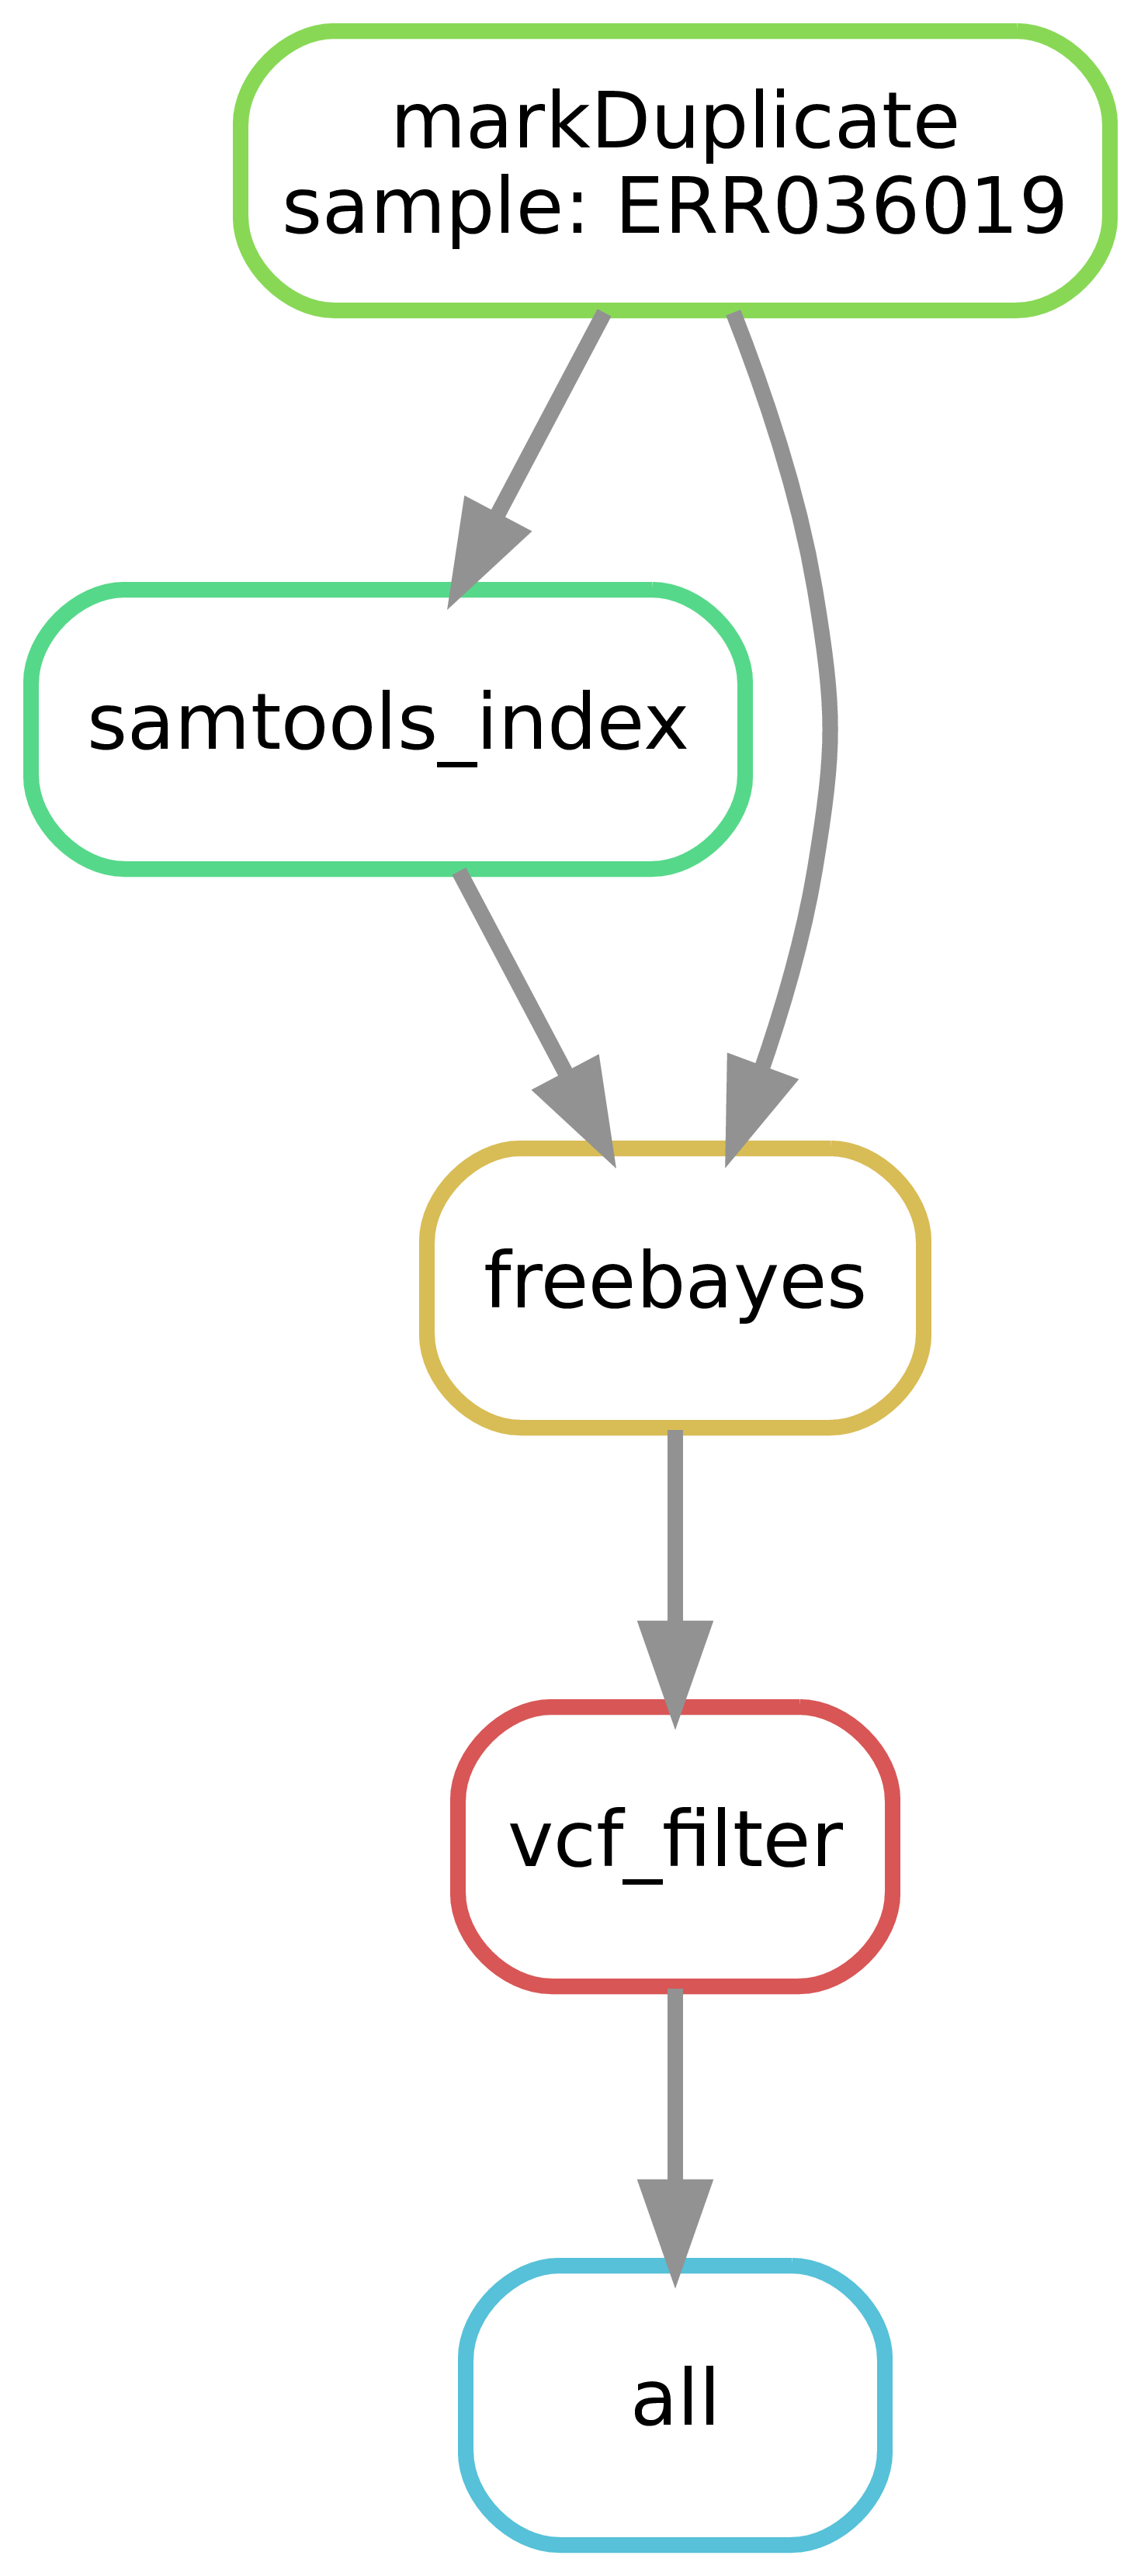
\includegraphics[scale=0.05]{dag_one_sample.png}
    \end{center}
\end{frame}

\section{References}

\begin{frame}
    \frametitle{References}
    \begin{itemize}
        \item Snakemake website:
        \begin{itemize}
            \item {\tiny https://bitbucket.org/snakemake/snakemake/wiki/Home}
        \end{itemize}
        \item Useful information:
        \begin{itemize}
            \item {\tiny http://slides.com/johanneskoester/deck-1}
            \item {\tiny http://snakemake.bitbucket.org/snakemake-tutorial.html}
            \item {\tiny http://slowkow.com/notes/snakemake-tutorial/}
            \item {\tiny http://watson.nci.nih.gov/{\textasciitilde{}}sdavis/blog/flexible\_bioinformatics\_pipelines\_with\_snakemake/}
        \end{itemize}
        \item Advanced example:
        \begin{itemize}
            \item {\tiny https://github.com/sequana/sequana/tree/master/pipelines/variants}
        \end{itemize}
        \item Enable syntax in vim for Snakemake
        \begin{itemize}
            \item {\tiny http://tinyurl.com/zm4b6c4}
        \end{itemize}
    \end{itemize}
\end{frame}

\section{Question}

\begin{frame}[fragile]
    \frametitle{Additional keywords}
    \begin{description}
        \item[threads] Set the number of threads needed
        \item[log] Set a log file for a rule
    \end{description}
    \begin{block}{Snakefile}
        \begin{lstlisting}
rule bwa_mapping:
    input:
        ref = "genome.fa",
        fastq = "sample_A.fastq.gz"
    output:
        "mapped_sample/sample_A.bam"
    threads: 8
    log:
        "logs/bwa_mapping/sample_A.log"
    shell:
        """
        (bwa mem -t {threads} {input.ref} {input.fastq} | \
        samtools view -Sb - > {output}) 2> {log}
        """
        \end{lstlisting}
    \end{block}
\end{frame}

\begin{frame}[fragile]
    \frametitle{Cluster special features}
    \begin{itemize}
        \item Snakemake generates log files with stdout and stderr of your jobs
            \begin{lstlisting}
            \end{lstlisting}
        \item Your current jobs are displaying with qstat
            \begin{lstlisting}
# ddesvill@bic ~/Test_fastq_dir > qstat
job-ID  prior   name       user         state submit/start at 
queue                          slots ja-task-ID 
-------------------------------------------------------------------------------
----------------------------------
3781631 0.63541 snakejob.b ddesvill     r     03/23/2016 12:17:04 
pf4@bic-n119.cluster.pasteur.f     1        
3781632 0.63541 snakejob.b ddesvill     r     03/23/2016 12:17:04 
pf4@bic-n119.cluster.pasteur.f     1        
3781633 0.63541 snakejob.b ddesvill     r     03/23/2016 12:17:04 
pf4@bic-n106.cluster.pasteur.f     1        
3781634 0.63541 snakejob.b ddesvill     r     03/23/2016 12:17:04 
pf4@bic-n422.cluster.pasteur.f     1        
3781635 0.63541 snakejob.b ddesvill     r     03/23/2016 12:17:04 
pf4@bic-n422.cluster.pasteur.f     1
            \end{lstlisting}
    \end{itemize}
\end{frame}

\begin{frame}[fragile]
    \frametitle{What happens when the snakemake is interrupted}
    \begin{itemize}
        \item If you stop your snakemake (i.e. ctrl+c):
        \begin{lstlisting}[language={}]
Terminating processes on user request.
Will exit after finishing currently running jobs.
Removing output files of failed job samtools since they might be corrupted:
reference.fa.fai
        \end{lstlisting}
        \item On the cluster, the current job is not kill
        \item If you close your shell (Crash simulation):
        \begin{lstlisting}[language={}]
IncompleteFilesException:
The files below seem to be incomplete. If you are sure that certain files are 
not incomplete, mark them as complete with

    snakemake --cleanup-metadata <filenames>

To re-generate the files rerun your command with the --rerun-incomplete flag.
Incomplete files:
ERR036019_unsort.bam
        \end{lstlisting}
        \item We can rerun the snakemake with \lstinline[basicstyle=\small\ttfamily]{--rerun-incomplete}.
    \end{itemize}
\end{frame}

\end{document}
